{\color{red}

TD write
- background:
    - sde ito
- pinns
    -x fourier features
    - samping: Euler Maruyama
    - score pinns
    - optimization strats notes
    - torch basics for pinns
    - ? nn basics - bs, backprop, ad (can add in later)
    - ? lbfgs
        - needs a fixed set of points
        - slowly change points during training

TD impl:
    - causal nope - my causal sampling yes
    - lbfgs on existing good runs
    - save runs to diploma-sketchbook case1-..

experiments
    - try score pinns and lbfgs on cluster
    - do large gs in d=3 for each case
        - sampling - trajs / latin
        - causal weighting
        - loss weighting - fixed vs adaptive

pavelka
    - sent pinn chapter
    - ask sde ito background public
}

\chapter{Abstract}


Partial differential equations are ...


Solving the diffusion equation using machine learning in higher dimension


\textbf{Keywords}:
partial differential equations,
diffusion equations,
Fokker-Planck,
curse of dimensionality,
scientific machine learning,
PINNS,
sparse grids combination technique,



\chapter{Introduction}

PDEs for modelling physical phenomena

curse of dimensionality

Machine learning in Scientific computing

Partial differential equations (PDEs) are essential mathematical 
tools for describing complex natural phenomena and engineering sys-tems
Traditional numerical meth-ods, such as the finite element method (FEM)
and the finite difference method (FDM), rely on spatial and temporal discretization to ap-proximate solutions by
constructing fine computational meshe
\cite{systematic_review}

increasingly used for modeling and simulating physical systems
despite some empirical success, PINNs are still facing many challenges
that define open areas for research and
further methodological advancements.
In recent years, there have been numerous studies focusing on improving the
performance of PINNs, mostly by
- neural network architectures
\cite{experts_guide}
fPINNS, XPINNS, varPINNS, ...


Most physical and engineering problems can be described by partial differential equations (PDEs),
which are typically solved using numerical methods such as the finite difference method and the finite element method.
However, conventional numerical discretization approaches face significant challenges in terms of computational efficiency
and convergence speed when dealing with complex nonlinear PDEs, such as high-
dimensional nonlinear PDEs, stiff PDEs, PDEs with complex boundary conditions or irregular geometries,
and multi-scale PDEs. Recently, physics-informed neural networks (PINNs) have emerged as a transforma-
tive methodology for solving complex PDEs by integrating physical laws intrinsically into deep learning architectures.
While PINNs effectively overcome mesh dependency and dimensionality constraints inherent in traditional numerical methods,
they still encounter persistent challenges related to training convergence and generalization robustness
\cite{systematic_review}

In the past few years, solving PDEs using machine and deep learning methods has emerged as a new and rapidly growing field of scientific machine learning.
Leveraging the universal approximation theorem \cite{uni_approx} and high expressivity of neural networks, the 

first by Lagaris et. at. \cite{lagaris}

Karniadakis in 2019 changes the game \cite{comprehensive}

climate modelling etc.


data + physs loss
solve inverse problems - value of a fucntion or a coefficient from the data

The 2019 publication by Karniadakis et al. was the seminal work that brought about the 
In combine machine learning with partial differential equation is a unique and simple way that was intuitive to both the machine learning and pde solving communities.
https://www.sciencedirect.com/science/article/abs/pii/S0021999118307125

flexibility of the arch


We focues on semi large dims

very large dims possible with
- 100s 1000s but sol at a point:

for very high dims
- multilevel picard method
- deep backward storchastic eq?
- deep galerkin
on the machine learning side

and feynman-kac monte carlo formulation


no systematic or even mention of existing sparse grids approach

here: diffusin eq. - spread - fokker planck, etc.
commonly probabilistic setting.
high-dimensionality naturally arrises in FP

Sparse grids
- basically FD but on carfully chosed low discret points meshes
- by on bounded seconds ders able to make tradeoff tham make it possible to scale to higher dims


This thesis is structured as follows.
First, backgroung on diffusion pdes and stochasic differential equations
Issues we encounter when naively scaling to higher dimensions
Sparse grids
feed-forward neural networks
PINNs - specifics etc and simple experiments demostraining they scaling to higher dims
Results:
simple heat eq
more challenging smoluchowski
initial conditions uhlenbeck processes.

\chapter{Introduction 0}

%% PDEs and diffusion pdes
Partial differential equations are one of the core tools in mathematical physics,
modelling wide range of physical and engineering phenomena.
%including heat transfer, diffusion, fluid flow, wave propagation, biological systems, etc.
An important subclass form diffusion-type equations, describing the evolution of quantities
that spread over time, such as temperature, concentration,
probability density, or chemical particles in a medium.
Specific examples include the heat equation, the diffusion equation, and the Fokker-Planck equation.

%% standard mesh FEM etc
The standard approaches for solving such equaitons numerically
discretinze the domain before . FD, FEM, FVM. Those method are a de facto standard
for low-dimensional problems, and here good convergence estimates.
However, they suffer from the curse of dimensionality,
as scaling them up to higher dimensions exponentially rises the set of discretization points.
Thus quickly approaching the memery limitation of existing hardware.

%% SG
Several approaches have been developed to combat this challenge.
One of which are sparse grids and notably, the sparse grid combination technique.
Sparse grids combination technique circumvents the curse of dimensionality
by constructing a combinations of lower-dimensional grids,
thus avoiding the full tensor-product construction.
Under suitable smoothness assumptions on the solution (smoothening effect of parab?), they provide
a compromise between approximation accuracy and computational cost, making
them attractive for moderately high-dimensional problems.
Sparse grids retain a strong connection to classical, and the formulation of the combiantion technique
allows reusing exisitng solvers, can run in parallel.

%% Scientific machine learnaing
From the other directiion, scientific machine learning active research field.
THe universal approximation theorem [3] guarantees that, under mild assump-
tions on the activation function, a sufficiently wide feed-forward network can
approximate any continuous function on a compact domain to arbitrary accuracy.
As such neural networks are capable of representing complicated functions.
flexinble
now not only empirical, but also theoretical developments

%% PINNS history
Early neural-network approaches to differential
equations were first proposed by Lagaris et al. [4] in 1999.
However, it was not until 2019, when
the work of Raissi, Perdikaris, and Karniadakis [5] introtion fo physics-informed neural networks
that caused large interest in teh field.

%% PINNS basic
One of the main advantages of PINNs is their simplicity and integraion into the
existing neural network formulation.
When compared to standard solveer, PINNs are mesh-free formulation. Instead
of constructing a full computational grid, the PDE residual is evaluated at selected
collocation points. This gives PINNs a natural appeal for high-dimensional
problems, where traditional mesh-based methods suffer from rapidly increasing
computational cost.s

%% modern PINNS
Nevertheless, PINNs also have important limitations. Their performance
depends on the choice of network architecture, sampling strategy, optimization
method, and weighting of the different loss terms.
Although many new model arch variants and extensions have been proposed, including
variants such as fPINNs, XPINNs, and variational PINNs, 
the reliable and efficient use of PINNs in higher-dimensional
settings remains an active area of research

%% This thesis goal:
This thesis investigates the use of machine learning methods for solving
diffusion-type partial differential equations in moderate-higher dimensional setting.
These problems are especially relevant
because probability density functions often live in high-dimensional state spaces.

%% This thesis struct:
The first chapters introduce the
mathematical background of diffusion equations, stochastic differential equations,
and Fokker-Planck equations.
Sparse grids and sparse grid combination technique
After that, feed-forward neural networks and physics-
7informed neural networks are presented
The numerical part of the thesis considers selected diffusion-type problems
including the heat equation, the Smoluchowski equation, to Ornstein-Uhlenbeck processes.
These results are used to evaluate the
accuracy, scalability, and limitations of the considered methods.
The results are analyzed with respect to accuracy, computational cost,
and scalability in higher dimensions.


\chapter{Introduction III}

The numerical solution of partial differential equations in high-dimensional spaces is one of the central challenges in modern scientific computing. Partial differential equations are used to model a wide range of physical and engineering phenomena, including heat transfer, diffusion, fluid flow, wave propagation, and stochastic dynamics. Among these models, diffusion equations are of particular importance because they describe the spreading of quantities in time and space. Closely related equations, such as the Fokker--Planck equation, also describe the evolution of probability densities associated with stochastic differential equations.

In low dimensions, diffusion equations can often be solved accurately using classical numerical methods. Finite difference methods and finite element methods approximate the solution by discretizing the computational domain and replacing the continuous problem by a finite-dimensional system. These methods are mathematically well understood and have been successfully applied in many areas of science and engineering. However, their direct extension to higher dimensions is severely limited by the curse of dimensionality. If a uniform grid with $n$ points in each coordinate direction is used in a $d$-dimensional domain, the total number of grid points is $n^d$. Even for moderate values of $n$ and $d$, this number becomes prohibitively large.

This dimensional scaling is not only a technical inconvenience, but a fundamental obstacle for many applications. High-dimensional diffusion and Fokker--Planck equations arise naturally when modelling systems with many degrees of freedom. Examples include molecular systems, interacting particle models, stochastic control, uncertainty quantification, and financial mathematics. In such problems, the unknown solution may represent a probability density over a high-dimensional state space. Solving the corresponding PDE on a full grid is usually impossible, and alternative approximation strategies are required.

Several approaches have been developed to address this difficulty. On the classical numerical side, sparse grids provide one way to reduce the cost of high-dimensional approximation. Instead of using all points of a full tensor-product grid, sparse grid methods select or combine lower-dimensional grid structures in a way that preserves much of the approximation power while using significantly fewer degrees of freedom. The sparse grid combination technique is especially attractive because it constructs an approximation from a linear combination of solutions on several anisotropic grids. For sufficiently smooth problems, sparse grids can reduce the computational complexity compared with full-grid methods and are therefore well suited for moderately high-dimensional PDEs.

At the same time, machine learning has become increasingly important in scientific computing. Neural networks are capable of representing complicated functions and have been used successfully in many high-dimensional approximation tasks. This has motivated the development of neural-network-based methods for solving PDEs. Early work by Lagaris et al. \cite{lagaris} showed that neural networks could be used to approximate solutions of differential equations. More recently, physics-informed neural networks (PINNs) have attracted significant attention, especially following the work of Raissi, Perdikaris, and Karniadakis \cite{comprehensive}. PINNs approximate the unknown solution by a neural network and train it by minimizing a loss function that includes the residual of the PDE as well as boundary and initial condition errors.

The key idea behind PINNs is to combine data-driven approximation with physical constraints. The governing equation is not treated as external information, but is built directly into the optimization problem. This makes PINNs flexible and relatively easy to apply to different PDEs. They can be used for forward problems, where the equation and parameters are known, as well as inverse problems, where unknown coefficients or functions are inferred from data. Since the method does not require a fixed mesh, it is particularly appealing for problems where mesh generation is difficult or where the dimension is too large for standard discretization.

Nevertheless, PINNs also have important limitations. Their performance depends on the choice of network architecture, sampling strategy, optimization method, and weighting of the different loss terms. In practice, PINNs may have difficulties with convergence, generalization, boundary accuracy, stiffness, and multiscale behaviour. Although many improved variants have been proposed, including domain-decomposition methods, variational PINNs, fractional PINNs, and extended PINNs \cite{experts_guide}, the efficient and reliable solution of higher-dimensional PDEs remains an open research problem \cite{systematic_review}.

This thesis focuses on solving diffusion equations using machine learning methods in higher dimensions. The aim is not only to apply physics-informed neural networks to diffusion-type problems, but also to understand their behaviour in comparison with structured numerical approaches such as sparse grids. The thesis is concerned with semi-high-dimensional problems, where full-grid discretization is already expensive, but where systematic numerical experiments are still possible.

The diffusion equation is used as a starting point because it is mathematically fundamental and allows clear evaluation of numerical behaviour. More challenging equations, such as the Smoluchowski equation and Fokker--Planck equations related to Ornstein--Uhlenbeck processes, are then considered to study problems with stronger probabilistic motivation. These models provide a natural setting for investigating how neural networks and sparse grid techniques behave as the dimension increases.

The structure of the thesis is as follows. The first chapters introduce the mathematical background of diffusion equations, stochastic differential equations, and Fokker--Planck equations. The curse of dimensionality is then discussed, with emphasis on why standard discretization methods become impractical in higher dimensions. The thesis next introduces sparse grids and the sparse grid combination technique. After that, feed-forward neural networks and physics-informed neural networks are presented. The final chapters contain numerical experiments for selected diffusion-type problems, followed by a discussion of the accuracy, computational efficiency, and scalability of the methods considered.



\chapter{Introduction II}

Many physical and engineering processes are governed by partial differential equations (PDEs). These equations describe how quantities evolve in space and time and are used to model phenomena such as heat conduction, diffusion, fluid motion, wave propagation, and transport processes. Diffusion equations form a particularly important class of PDEs, since they describe the spreading or smoothing of a quantity over time. They also appear in probability theory, where the Fokker--Planck equation describes the time evolution of probability densities associated with stochastic differential equations.

For decades, PDEs have been solved primarily by classical numerical methods, including finite difference methods, finite element methods, and finite volume methods. These methods approximate the continuous problem by discretizing the computational domain and solving a finite-dimensional algebraic system. In low spatial dimensions, they are highly successful and form the basis of many scientific and engineering simulations. However, their applicability becomes limited when the dimension of the problem increases. A full tensor-product discretization requires a number of grid points that grows exponentially with the dimension, leading to the well-known curse of dimensionality. This makes many high-dimensional PDEs computationally infeasible using standard discretization techniques.

The curse of dimensionality is especially relevant for diffusion-type equations in probabilistic settings. For example, Fokker--Planck equations often describe probability densities over the state space of a stochastic system. If the underlying system has many degrees of freedom, the associated PDE becomes high-dimensional. Such equations occur in statistical physics, molecular dynamics, finance, uncertainty quantification, and other areas. Although Monte Carlo and stochastic methods can sometimes avoid solving the full density equation directly, there remains strong interest in deterministic and machine-learning-based methods that can approximate high-dimensional PDE solutions more efficiently.

Scientific machine learning has recently become an active research field at the intersection of numerical analysis, machine learning, and scientific computing. Neural networks offer a flexible way of approximating functions in high-dimensional spaces, and their success in data-driven modelling has motivated their use for solving differential equations. Early neural-network approaches to differential equations were proposed by Lagaris et al. \cite{lagaris}, while the modern development of physics-informed neural networks (PINNs) was strongly influenced by the work of Raissi, Perdikaris, and Karniadakis \cite{comprehensive}. PINNs solve PDEs by representing the unknown solution with a neural network and training it to satisfy the governing equation, boundary conditions, and initial conditions through a physics-informed loss function.

One of the main advantages of PINNs is their mesh-free formulation. Instead of constructing a full computational grid, the PDE residual is evaluated at selected collocation points. This gives PINNs a natural appeal for high-dimensional problems, where traditional mesh-based methods suffer from rapidly increasing computational cost. PINNs can also incorporate observational data, which makes them suitable not only for forward problems but also for inverse problems, such as estimating unknown parameters, coefficients, or source terms from measurements.

However, despite their empirical success, PINNs are not a complete solution to the challenges of high-dimensional PDEs. Their training can be unstable, slow, or sensitive to hyperparameter choices. The balance between the PDE residual, boundary conditions, initial conditions, and possible data terms can strongly affect the final approximation. Furthermore, PINNs may struggle with stiff systems, multiscale behaviour, sharp gradients, complicated geometries, or high-dimensional domains \cite{systematic_review}. Many recent studies therefore focus on improving PINN performance through modified architectures, adaptive sampling strategies, domain decomposition, variational formulations, or fractional and extended PINN variants \cite{experts_guide}.

This thesis studies the solution of diffusion equations using machine learning methods in higher dimensions. The main objective is to investigate how physics-informed neural networks behave when applied to diffusion-type PDEs beyond the simplest low-dimensional cases. The thesis focuses on semi-high-dimensional settings, where the dimension is sufficiently large to expose the limitations of classical full-grid methods, but still manageable enough to allow controlled numerical experiments and comparisons.

A second important component of this thesis is the sparse grid combination technique. Sparse grids provide a classical numerical approach designed to reduce the cost of high-dimensional approximation. Instead of using a full tensor-product grid, sparse grid methods combine solutions computed on anisotropic lower-resolution grids. Under appropriate smoothness assumptions, this can significantly reduce the number of degrees of freedom while maintaining good approximation accuracy. This makes sparse grids a useful reference point between classical discretization methods and neural-network-based methods.

The thesis combines these perspectives to study diffusion-type PDEs from both numerical and machine-learning viewpoints. It begins with the mathematical background of diffusion equations, stochastic differential equations, and Fokker--Planck equations. It then discusses the curse of dimensionality and explains why direct discretization becomes problematic in higher dimensions. After that, sparse grids, feed-forward neural networks, and physics-informed neural networks are introduced. The numerical part of the thesis considers model problems such as the heat equation, the Smoluchowski equation, and examples related to Ornstein--Uhlenbeck processes. These experiments are used to evaluate the accuracy, scalability, and limitations of the considered methods.



\chapter{Introduction I}

Partial differential equations (PDEs) are among the most important mathematical tools for modelling physical, biological, and engineering systems. They arise naturally in the description of transport processes, fluid flow, heat transfer, quantum mechanics, population dynamics, and many other phenomena. Among them, diffusion-type equations play a particularly central role, as they describe the evolution of quantities that spread over time, such as temperature, concentration, probability density, or chemical particles in a medium. Important examples include the heat equation, the diffusion equation, and the Fokker--Planck equation, which appears in the probabilistic description of stochastic dynamical systems.

Classical numerical methods for solving PDEs include the finite difference method, the finite element method, and finite volume methods. These approaches rely on discretizing the spatial and temporal domain and approximating the solution on a computational mesh. For low-dimensional problems, such methods are well established and highly effective. However, their computational cost increases rapidly as the dimension of the problem grows. This phenomenon, commonly known as the curse of dimensionality, makes the direct application of standard grid-based numerical methods infeasible for many high-dimensional PDEs. In particular, equations such as high-dimensional diffusion equations or Fokker--Planck equations require a number of discretization points that grows exponentially with dimension when full tensor-product grids are used.

In recent years, machine learning methods have emerged as a promising alternative for solving PDEs in scientific computing. Neural networks are flexible function approximators, and their expressive power makes them suitable candidates for representing high-dimensional solution functions. Building on the universal approximation theorem \cite{uni_approx}, early work by Lagaris et al. \cite{lagaris} proposed neural-network-based approaches for solving differential equations. Later, physics-informed neural networks (PINNs) became one of the most influential frameworks in this area, especially after the work of Raissi, Perdikaris, and Karniadakis \cite{comprehensive}. PINNs incorporate the governing physical laws directly into the loss function by penalizing the residual of the differential equation together with boundary and initial conditions. This allows the method to solve PDEs without requiring a traditional mesh and makes it applicable both to forward and inverse problems.

Despite their flexibility, PINNs still face several important challenges. Their performance can strongly depend on the neural network architecture, the choice of collocation points, the relative weighting of loss terms, and the optimization procedure. Training can become difficult for stiff equations, multiscale problems, complex boundary conditions, or higher-dimensional domains. Although many extensions have been proposed, including variants such as fPINNs, XPINNs, and variational PINNs \cite{experts_guide}, the reliable and efficient use of PINNs in higher-dimensional settings remains an active area of research \cite{systematic_review}.

This thesis investigates the use of machine learning methods for solving diffusion-type equations in higher dimensions. The main focus is on semi-high-dimensional problems, where the dimension is large enough for classical full-grid discretizations to become expensive, but still within a range where structured numerical comparisons are possible. The thesis considers diffusion equations and related Fokker--Planck-type models, which naturally arise in probabilistic settings and stochastic differential equations. These problems are especially relevant because probability density functions often live in high-dimensional state spaces.

In addition to neural-network-based methods, this thesis also considers sparse grids and the sparse grid combination technique. Sparse grids can be understood as carefully selected combinations of lower-dimensional grids that avoid the full tensor-product construction. Under suitable smoothness assumptions, they provide a compromise between approximation accuracy and computational cost, making them attractive for moderately high-dimensional PDEs. Unlike fully mesh-free neural network approaches, sparse grids retain a strong connection to classical numerical discretization while reducing the dimensional scaling of the problem.

The goal of this thesis is therefore to compare and study approaches for solving diffusion equations in higher dimensions, with particular attention to the interaction between classical numerical methods, sparse grid techniques, and physics-informed neural networks. The work explores how these methods behave as the dimension increases, what difficulties arise when scaling standard approaches, and how machine learning can be used to approximate solutions of diffusion-type PDEs.

The thesis is structured as follows. First, the necessary mathematical background on diffusion equations, Fokker--Planck equations, and stochastic differential equations is introduced. Next, the curse of dimensionality and the difficulties of naively scaling classical discretization methods to higher dimensions are discussed. The following chapters introduce sparse grids, feed-forward neural networks, and the PINN framework. Numerical experiments are then presented, starting with simple heat equation examples and continuing to more challenging models such as the Smoluchowski equation and problems related to Ornstein--Uhlenbeck processes. Finally, the results are analyzed with respect to accuracy, computational cost, and scalability in higher dimensions.






\chapter{Feed-forward neural networks}
%{\color{red}
%FOR ME: core concepts to cover:
%
%- activations relu vs tanh
%
%- backpropagation
%
%- batch size
%}


Fundamentaly, neural networks are parametric function approximators.

Since their inception in .... numerous different competing architercure emerged
each design to a particular problem

more complex
- recursive
- transformer

focues on the simple original one

The universal approximation theorem \cite{uni_approx} guarantees that, under mild assumptions on the activation function, a sufficiently wide feed-forward network can approximate any continuous function on a compact domain to arbitrary accuracy.
Their power lies in their simplicity and the flexibility with which the architecture can be tailored to the specific problem at hand.
The downside of such flexibility is that it introduces a large number of architectural and hyperparametric choices, and identifying a good combination is often not trivial.

\subsection{Architecture}

A feed-forward neural network, sometimes also called a Multil-Layer Perceptron, is a composition of affine transformations connected by nonlinearities called \emph{activation functions}, denoted as $\sigma$ (e.g.\ $\tanh$, ReLU,...).

A single hidden layer transforms its input $x \in \mathbb{R}^{d_{l-1}}$ as
$$
h^{(l)}(x) = \sigma\!\bigl(W^{(l)} x + b^{(l)}\bigr),
\qquad W^{(l)} \in \mathbb{R}^{d_l \times d_{l-1}}, \; b^{(l)} \in \mathbb{R}^{d_l},
$$
where $W^{(l)}$ and $b^{(l)}$ are the \emph{weights} and \emph{biases} of the $l$-th layer.

Stacking $L$ such layers and applying a final activation $a$ gives
$$
\mathcal{N}_\theta : \mathbb{R}^{d_{\mathrm{in}}} \to \mathbb{R}^{d_{\mathrm{out}}}
\qquad
\mathcal{N}_\theta = a \circ h^{(L)} \circ \cdots \circ h^{(1)}
$$
where $\theta = \{W^{(l)}, b^{(l)}\}_{l=1}^{L+1}$ is the set of all trainable parameters.

The nonlinearity $\sigma$ is essential: without it, the above given composition of hidden layes would collapse into a single linear affine map and the network's expressive power would be that of linear regression.

The number of hidden layers $L$ (\emph{depth}) and the layer sizes $d_l$ (\emph{width}) together control the capacity, commonly noted as expressive power, of the model.




\subsection{Training}

Training a NN amounts to solving an optimization problem in the parameter space of $\theta$.

Given training data $\{(x_i, y_i)\}_{i=1}^N$ and a loss functional $\ell(\theta)$ measuring the difference between network predictions $\mathcal{N}_\theta(x_i)$ and targets $y_i$ (most commonly using the mean squared error as the metric), one seeks to find
$$
\theta^{\star} = \arg\min_{\theta}\, \ell(\theta)
$$
Because $\ell$ is in general non-convex and high-dimensional (the networks we will consider have on the order of $10^4$--$10^7$ parameters),
the minimization is carried out by first-order iterative methods, starting from \emph{(stochastic) gradient descent}
$$
\theta \leftarrow \theta - \eta\, \nabla_\theta \ell(\theta)
$$
with learning rate $\eta > 0$. In practice, more complex variants such as Adam \cite{king_adam} are preferred, as they converge faster and are less sensitive to the choice of $\eta$.

A core part of the the training pipeline that enables efficient compuation of the gradient w.r.t the network parameters $\theta$ is \emph{automatic differentiation} (AD).
Since the ouput of $\mathcal{N}_\theta$ is computed from a finite sequence of elementary operations whose derivatives are known analytically, ($\frac{d}{dx}(x\cdot w) = w, \frac{d}{dx}\tanh{x} = sech^2 x$, etc.),
we can simply apply the chain rule to obtain $\nabla_\theta \ell$ exactly (up to floating-point round-off).

% note: forward and backpropagation

As we will see in the following section, this very same mechanism is exploited by PINNs to differentiate the network with respect to its spatial and temporal inputs, thus computing the individual terms in the given partial differential equation.

The full training algorihm for feed-forward neural networks can thus summarized as so:

\begin{algorithm}[H]
\caption{Full-Batch Gradient Descent}
\begin{algorithmic}[1]
    \Require $\mathcal{N}_{\theta}:\mathbb{R}^{d_{in}}\to\mathbb{R}^{d_{out}}$, training data $\{(x_i, y_i)\}_{i=1}^{N}$, number of epochs $E$, learning rate $\mu$
    \State \textbf{Initialize} network parameters $\theta$
    \For{epoch $= 1, \dots, E$}
        \State Randomly shuffle the training data
        \State \textbf{Forward pass:} compute $\hat{y}_i = \mathcal{N}_\theta(x_i), \:\forall i$
        \State \textbf{Compute loss:}
        $\ell(\theta) = \dfrac{1}{N}\displaystyle\sum_{i=1}^N
                \bigl(\hat{y}_i - y_i\bigr)^2$
        \State \textbf{Backward pass:} compute $\nabla_\theta \ell$ via backpropagation
        \State \textbf{Update:} $\theta \leftarrow \theta - \eta\,\nabla_\theta \ell$
    \EndFor
    \State \Return $\theta$
\end{algorithmic}
\end{algorithm}

This algorihm is called a \emph{full-batch gradient descent}, since it processes the entire training set simultaneously as a one single batch in a single step.
However, in cases where the dataset is too big to precess all at once, we split it into mutliple batches and proceed iteratively until we go thus process the entire dataset.
\cite{goodfellow}


\begin{algorithm}[H]
\caption{Mini-Batch Gradient Descent}
\begin{algorithmic}[1]
    \Require $\mathcal{N}_{\theta}:\mathbb{R}^{d_{in}}\to\mathbb{R}^{d_{out}}$, training data $\{(x_i, y_i)\}_{i=1}^{N}$, number of epochs $E$, batch size $B$, learning rate $\mu$
    \State \textbf{Initialize} network parameters $\theta$
    \For{epoch $= 1, \dots, E$}
        \State Randomly shuffle the training data
        \State Divide the data into batches of size $B$
        \For{each batch $\mathcal{B} \subset \{1,\dots,N\}$, $|\mathcal{B}|=B$}
            \State \textbf{Forward pass:} compute $\hat{y}_i = \mathcal{N}_\theta(x_i)$ for $i\in\mathcal{B}$
            \State \textbf{Compute loss:}
            $\ell(\theta) = \dfrac{1}{B}\displaystyle\sum_{i\in\mathcal{B}}
                \bigl(\hat{y}_i - y_i\bigr)^2$
            \State \textbf{Backward pass:} compute $\nabla_\theta \ell$ via backpropagation
            \State \textbf{Update:} $\theta \leftarrow \theta - \eta\,\nabla_\theta \ell$
        \EndFor
    \EndFor
    \State \Return $\theta$
\end{algorithmic}
\end{algorithm}

In the algorihm above, the subset $\mathcal B$ of the training data is called a \emph{batch}, and $B$ is called a \emph{batch size}.

The deciding factor between using a single large batch or set of smaller ones is not just the size of the dataset.
For exmaple, small batch sizes are more noisy and can thus offer a regulizing effect for the network - enabling it to escape local miniam. On the other hand, large batch sizes give a more accurrate estimate of the gradient.
The choice also depends on the hardware, espetially when using GPUs - as they are quite limited by VRAM, and their architecture makes them prefer a power of 2 batchsize. 
\cite{goodfellow}



\chapter{PINNs I}

Physics-informed neural networks (PINNs) are a class of neural-network-based methods for solving problems governed by differential equations. They combine the approximation capabilities of feed-forward neural networks with prior knowledge about the physical or mathematical structure of the system under consideration. This prior knowledge is usually given in the form of a differential equation, together with suitable initial and boundary conditions.

The central idea of PINNs is to represent the unknown solution of a differential equation by a neural network. Instead of training the network only on labelled input-output data, the network is trained to satisfy the governing equation itself. This is achieved by constructing a loss function that penalizes the residual of the differential equation, as well as deviations from the prescribed initial and boundary conditions. In this way, the physical model becomes part of the training objective.

Before the development of PINNs, neural networks were already used in scientific computing mainly as flexible approximators of available data. In such settings, the network learns a mapping from input data to output data, but it does not necessarily respect the physical laws that generated the data. PINNs extend this idea by incorporating a priori domain knowledge directly into the learning process. As a result, the network is not only fitted to data, but is also constrained by the underlying mathematical model.

In the context of PDEs, the neural network takes the independent variables, such as space and time, as inputs and returns an approximation of the solution. For example, for a time-dependent problem in a spatial domain $\Omega \subset \mathbb{R}^d$, one may define a neural network
\[
    u_\theta : \Omega \times [0,T] \to \mathbb{R},
\]
where $\theta$ denotes the trainable parameters of the network. The goal is to choose $\theta$ such that $u_\theta$ approximates the true solution $u$ of the PDE.

A general PDE problem can be written in the form
\[
    \mathcal{N}[u](x,t) = 0, \qquad (x,t) \in \Omega \times (0,T],
\]
together with boundary and initial conditions
\[
    \mathcal{B}[u](x,t) = 0, \qquad (x,t) \in \partial \Omega \times (0,T],
\]
and
\[
    u(x,0) = u_0(x), \qquad x \in \Omega.
\]
Here, $\mathcal{N}$ denotes the differential operator defining the PDE, and $\mathcal{B}$ denotes the boundary operator. In the PINN framework, the exact solution $u$ is replaced by the neural network approximation $u_\theta$. The PDE residual is then given by
\[
    r_\theta(x,t) = \mathcal{N}[u_\theta](x,t).
\]

The derivatives appearing in the residual are computed using automatic differentiation. This is one of the main advantages of PINNs, since it allows the differential equation to be evaluated directly from the neural network representation without constructing finite difference stencils or finite element basis functions. The resulting residual can be evaluated at a set of collocation points sampled from the computational domain.

The loss function typically consists of several terms. A common form is
\[
    \mathcal{L}(\theta)
    =
    \lambda_r \mathcal{L}_r(\theta)
    +
    \lambda_b \mathcal{L}_b(\theta)
    +
    \lambda_0 \mathcal{L}_0(\theta),
\]
where $\mathcal{L}_r$ is the residual loss corresponding to the PDE, $\mathcal{L}_b$ is the boundary loss, and $\mathcal{L}_0$ is the initial condition loss. The constants $\lambda_r$, $\lambda_b$, and $\lambda_0$ are weights that determine the relative importance of the different terms. If measurement data are available, an additional data loss term can also be included.

An important feature of PINNs is that they can be trained even when no labelled solution data are available. In that case, the method relies entirely on the governing equation and the prescribed initial and boundary conditions. This makes PINNs attractive for solving forward PDE problems, where the aim is to approximate the solution of a known equation. At the same time, PINNs can also be applied to inverse problems, where unknown parameters, coefficients, or source terms are inferred from partial observations.

From a computational point of view, PINNs fit naturally into the existing machine learning pipeline. The solution is represented by a standard feed-forward neural network, the residual is computed using automatic differentiation, and the parameters are optimized using gradient-based methods. This makes PINNs relatively flexible and easy to implement in modern deep learning frameworks.

However, PINNs also have important limitations. The optimization problem is often non-convex and can be difficult to solve. The accuracy of the method depends on the architecture of the network, the distribution of collocation points, the choice of optimizer, and the balance between the different loss terms. In higher-dimensional problems, training can become expensive and unstable, and the method may require careful tuning. For this reason, understanding the practical behaviour of PINNs is essential before applying them to more challenging diffusion-type equations.

The following sections describe the specific PINN architecture used in this thesis, the construction of the loss function, the sampling of collocation points, and the implementation details relevant to the numerical experiments.





\chapter{Phyics-Informed Neural Networks (PINNs)}


First introduces by Lagaris et. at. \cite{lagaris} in 1997,
and later reformulated by Karniadakis et. al., Physics-Informed Neural Networks combine
the architecture and training loop of traditional feed-forward neural networks
with the information about the physics governing the system under consideration.
This information is added in in a form of a specific loss function which the model is trained to minimize.

Pior to the introduction of PINNs, neural netoworks were used in the scientific computing
as interpolators of measurement data. 
In this context, the network learns a mapping from input data to output data,
but it does not necessarily respect the physical laws unterlying the phenomena.

The novel idea introduced by PINNs was to extend the loss function by an extra term incorporating the knowledge about the phycics.
As a result, the resulting network becomes less prone to overfitting, and is much more constrained by the physics.

On the other hand, such a formulation allow us to train the network even when no labelel measurement data are available.
In that case, the loss relies entirely on the governing equation and the prescribed initial and boundary conditions.
This feature makes them useful as differential equation solvers.

The main attractiveness of PINNs is that they fit naturally into the existing
machine learning pipeline. The solution is represented by a standard feed-forward
neural network, the residual is computed using automatic differentiation, and
the parameters are optimized using gradient-descent methods.
This makes PINNs relatively flexible and easy to implement in the existing deep learning frameworks.

However, PINNs also have important limitations.
The loss landscape in generally non-convex and the resulting optimization problem can be difficult to solve.
The accuracy of the method is very sensitive to the choice of hyperparameters, such as
on the architecture of the network,
the choice of optimizer,
the balance between the different loss terms,
and 
the distribution of training points.
This problem is even more pronounced in PINNs as we shall see later on.
In more complex settings, such as our higher-dimensional problems,
training can become expensive and unstable, and
the method may require careful tuning.
For this reason, understanding the
practical behaviour of PINNs is essential before applying them to more challenging
diffusion-type equations.

The following sections describe the specific PINN architecture used in this
thesis, the construction of the loss function, the sampling of collocation points,
and the implementation details relevant to the numerical experiments.




%We base our PINN architecture on a few crutial publications and based took the inspiration of our implemntation from some existing established codebases.
%Namely:
%\begin{itemize}
%    \item studies published by Karniadakis et. al, including
%    \begin{itemize}
%        \item HTE
%        \item SDGD
%    \end{itemize}
%    \item deepxde - rar
%\end{itemize}
%Needed to code from scratch - relatively novel field, no codebase has access to the latest architecutres combined that we wanted to explore - relevant to high dims
%
%physics-informed - PDE in the loss function
%
%diff eq in network, learns physics, dooes not overfit the training data:
%PINNs differ from traditional neural networks in their ability to incorporate a priori domain knowledge of the problem in the form of differential equations.
%This additional information enables PINNs to make more accurate predictions outside of the given measurement data.
%Furthermore, the additional physics knowledge regularizes the predicted solution in the presence of noisy measurement data, enabling PINNs to learn the true underlying signal rather than overfitting the noisy data.
%https://www.mathworks.com/discovery/physics-informed-neural-networks.html


\section{Architecture}
%{\color{red}
%- input dim
%- ouput dim
%- loss
%- diagram
%
%give general arch before moving to more specific ones
%
%vanilla pinn
%- feed forward
%- tanh activations - smooth derivatives
%- loss functions based on the physics - the PDE of the system
%- convergence to a glob min if sol unique, pde well-possed, NN expressive, and enough points
%
%- simple problem
%    - 100s-1000s pnts paired with lbfgs
%- more efficient - stoch grad desc
%}

The basic architecture of a physics-informed neural network
is commonly a standard feed-forward neural network as described in chapter 3.
The main differenting factor of PINNs is not the architecture itself,
but rather the construction of the loss and a few training specific details
depending on the differetial equation at hand.

Consider, for example, a system of the form
\begin{align}
\partial_t u(x,t) + \mathcal L(u;x,t) = 0& \quad\Omega\times(0,T)\\
u(x) = u_{ic}(x)& \quad\Omega\\
u(x,t) = u_{bc}(x,t)& \quad\partial\Omega\times(0,T)
\end{align}

where
$\Omega\subset\mathbb R^d$,
$\mathcal L$ is a general spatial differential operator, and $u_{bc}, u_{ic}$ are the given boundary and initial data.
Provided it exists, the solution of the PDE is then a mapping
$$
u: \Omega \times [0,T] \to \mathbb{R} \,.
$$

In the context of PINNs, we parametrize the solution by a neural network
$$
u_\theta : \Omega \times [0,T] \to \mathbb{R}
$$
where $\theta$ denotes the trainable parameters of the network.

Since the input consists of the spatial variable $x \in \mathbb{R}^d$ together with time $t \in \mathbb{R}$, the input dimension of the network is
$d_{\mathrm{in}} = d + 1$, and for a scalar PDE, the output dimension is $d_{\mathrm{out}} = 1$.

In the case where PDE existence theory guarantees a smooth solution,
we prefer a smooth activation function for the hidden layers,
generally a hyperbolic tangent, followed by a identity activation for the final output layer.
However, even in the case of initial / boundary data from $C(\Omega)$ whose first derivatives are discontinuous,
the hyperbolic tangent is the dominant choice in the literature.
% This is because the differential operator
Moreover, diffusion equaitons tend to smooth out any of discontinuous initial / boundary data.
Henceforth, we will only consider architectures with $\tanh$ activations.
%The choice of activation function is particularly important in PINNs. Since
%the network represents a solution of a differential equation, it is often necessary
%for the network output to be differentiable with respect to its inputs. For this
%reason, smooth activation functions are commonly preferred. A standard choice is
%the hyperbolic tangent activation function,

\begin{figure}
    \centering
    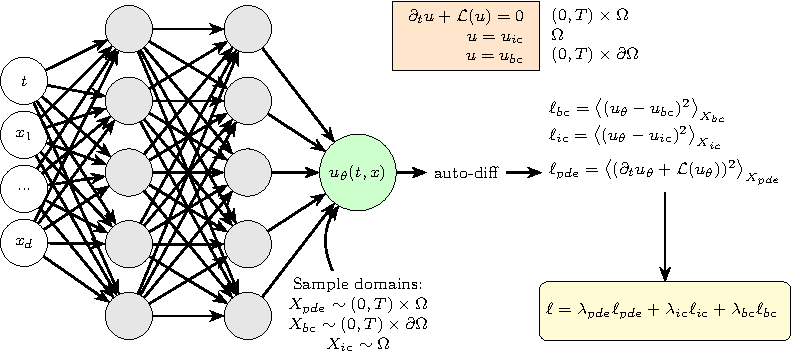
\includegraphics[width=150mm]{pinn_arch.pdf}
    \caption{}
    \label{fig:pinn_arch}
\end{figure}



\section{Residuum and Loss}
As previously mentioned,
the central feature separating physics-informed neural networks from other neural network based strategies for modelling differential equations
is the specific construction of the loss.

Returning to the system 5.1 above, we now define a PDE, BC, and IC \emph{residua} at a space time coordinate $(x,t)$ as
\begin{align*}
\mathcal R_{pde}(u;x,t) &= \partial_t u(x,t) + \mathcal L(u;x,t)\\
\mathcal R_{bc}(u;x,t) &= u(x,t) - u_{bc}(x,t)\\
\mathcal R_{ic}(u;x) &= u(x,0) - u_{ic}(x)
\end{align*}

Next, in our formulation of PINNs, the training data does not contain the target values $u_i$ for the inputs $(x_i,t_i)$,
as we don't have access to the solution $u$.
Instead, the training data only contain a set of points spanning the domain.
We call such a set of points a \emph{callocation set}, or just \emph{callocaiton points}.

Our dataset thus consist of three sets of callocation points, one for each domain
\begin{align*}
X_{pde}& := \{(x_i,t_i)\}_{i=1}^{N_{pde}} \subset (0,T)\times\Omega\\
X_{bc}& := \{(x_i,t_i)\}_{i=1}^{N_{bc}} \subset (0,T)\times\partial\Omega\\
X_{ic}& := \{x_i\}_{i=1}^{N_{ic}} \subset \Omega
\end{align*}
%Where the callocation points are either sampled beforehand or during training.

The loss the neural network then seeks to minimize is a linear combiantion
\begin{align*}
\ell = \lambda_{pde}\ell_{pde} + \lambda_{bc}\ell_{bc} + \lambda_{ic}\ell_{ic}
\end{align*}

where $\lambda_r>0$, and the individual losses are computed as a mean squared error of the residuum over the sample callocation points
\begin{align*}
\ell_{pde}\left(\theta;X_{pde}\right)
&= \frac{1}{N_{pde}}\sum_{i=1}^{N_{pde}} \big(\mathcal R_{pde}(u_\theta;x_i,t_i)\big)^2\\
\ell_{bc}\left(\theta;X_{bc}\right)
&= \frac{1}{N_{bc}}\sum_{i=1}^{N_{bc}} \big(\mathcal R_{bc}(u_\theta;x_i,t_i)\big)^2\\
\ell_{ic}\left(\theta;X_{ic}\right)
&= \frac{1}{N_{ic}}\sum_{i=1}^{N_{ic}} \big(\mathcal R_{ic}(u_\theta;x_i)\big)^2
\end{align*}

To aid in notation, the expression for the loss of a particular term, over a given callocation set $X_r:=\{\xi_i\}_{i=1}^{N_{r}}$, can be expressed more concisely, as
$$
\ell_{r}\left(\theta;X_r\right)
= \frac{1}{N_r}\sum_{i=1}^{N_{r}} \big(\mathcal R_{r}(u_\theta;\xi_i)\big)^2
%= \mathbb E \left[\big(\mathcal R_{r}(u_\theta;\xi_i)\big)^2\right]_{\xi_i\in X_r}
= \left\langle\big(\mathcal R_{r}(u_\theta;\xi_i)\big)^2\right\rangle_{\xi_i\in X_r}
$$


\section{Automatic differentiation (AD)}
{\color{red}

second der


}


So far, we haven't specified how the individual spatial and temporal derivatives
making up the PDE residuum are to be computed. Let us adress this now.

% We briefly touched on it when discussing feed forward neural networks.
As mentioned in chapter 4, during the training of neural networks,
we employ automatic differentiation to obtain the gradient of the loss function
with respect to the model weights.

In PINNs we reuse this strategy to calculate the gradient of the network w.r.t its input $(t,x)$,
$\nabla_{(t,x)} u_\theta(t,x)$, thus obtaining $\nabla_t u = \partial_t u$ and $\nabla_x u$.
We can repeat this procedure to obtain higher order derivatives.

Since its central nature in the of PINNs, lets us devote more time to understanding
what exactly is going on under the hood, as this knowledge will prove to be
crutial for scaling PINNs to high dimensional domains.

\subsection{Fundamentals}
Neural networks are composed of a elementary mathematical operations and activation functions.
The majority of the network is a compositoin of transformations units of the type
$$
h = \sigma(x^T W + b)
$$
where $W\in\mathbb R^{M\times N},b\in\mathbb R^N$ are parameters of the network and $x\in\mathbb R^M$ is some input

Lets now consider a case where all variables are scalars:
$$
h = \sigma(x w + b)
$$
We can interpret this calculation as a directed acyclic graph (DAG), see fig 1.

To calculate a gradient of the output of neural network with respect to some variable, lets say $x$
we just apply the chain rule multiple times:
$$
\frac{d h}{d x} = 
\frac{d h}{d z} 
\frac{d z}{d y} 
\frac{d y}{d x} 
$$
$$
\frac{\partial z}{\partial y} = 
$$


- decomposes into elementary operations
- uses chain rule
- exact up to machine precision



DAG - directed acyclic graph

Let us explore this further - as it will show be to for PINNS.
Building a computational graph during the forward pass as operations are performed
Tracking relationships between values through their operations
Computing gradients during the backward pass by applying the chain rule recursively


\subsubsection{Automatic differentiation in PINNs}

wrt to input - only need eval at point - not at neighborhood

graph in a graph in a graph??

how do they stack?

memory needs?


Diagrams:
- decompose the network into elem units
- forward vs reverse mode grad comp

\subsubsection{Implementation}
leaves and root
Function object
    - knows how to compute forward and also its der in backprop step
DAG - directed acyclic graph consisting of Funciton objects
leaves = input tensor
roots = output tensor

By tracing this graph from roots to leaves,
you can automatically compute the gradients using the chain rule.

The backward pass kicks off when `'.backward()`' is called on the DAG root. autograd then:
- computes the gradients from each $.grad_fn$,
- accumulates them in the respective tensor's .grad attribute
- using the chain rule, propagates all the way to the leaf tensors.

when doing backward propagation,
PyTorch accumulates the gradients,
i.e. the value of computed gradients is added to the
grad property of all leaf nodes of computational graph


\subsubsection{Automatic differentiation vs. Finite differences}

\cite{fd_ad}
FD for no hessian operators - laplace, grad, etc ??
- only 2 extra points - laplace stencil and central der

Training error the main issue for DF

- fd
    - mem cheaper
for second order diff operator:
    - ad and fd almost same training time
    - but observe training
    - different loss landscape
        - that one for ad better
    - ad:
        - lower residual tarining error
        - faster loss convergence

gradient-descent training kernel G for two-layer FFNN
AD and FD have similar large singular/eigenvalues, as FD approximates AD,
but FD produces relatively larger small singular/eigenvalues due to numerical differentiation artifacts
These small values matter because training is sensitive to the low end of the spectrum
- similar as when Ax=b - condition numer sigma max / sigma min

same problem, increase the number of neurons
the error rises linaerly
- need to increase n of steps





\section{Training}

{\color{red}

- sample once, epoch = 1 pass thought the dataset

- sample new data every step
}


The training regime is analogous to that of feed-forward neural network:


%Let us save the training data $\{(x_i,t_i)\}_{i=1}^{N_{pde}}$ as a tensor $\mathbf X_{pde}$ of size $(N_r,d+1)$

\begin{algorithm}[H]
\caption{Full-Batch Gradient Descent}
\begin{algorithmic}[1]
    \Require 
    \begin{itemize} 
    \item $u_\theta:\mathbb{R}^{d+1}\to\mathbb{R}$
    \item callocation sets $X_{pde}, X_{bc}, X_{ic}$
    \item weights $\lambda_{pde}, \lambda_{bc}, \lambda_{ic}$
    \end{itemize} 
    \State \textbf{Initialize} network parameters $\theta$
    \For{epoch $= 1, \dots, E$}
        \State Randomly shuffle the callocation points
        \State \textbf{Forward pass:}
        \begin{itemize} 
            \item $u_{pde,i} = u_\theta(x_i,t_i),\quad \forall(x_i,t_i)\in X_{pde}$
            \item $u_{bc,i} = u_\theta(x_i,t_i),\quad \forall(x_i,t_i)\in X_{bc}$
            \item $u_{ic,i} = u_\theta(x_i,0),\quad \forall x_i\in X_{ic}$
        \end{itemize} 
        \State \textbf{Calculate residua and loss:}
        \begin{itemize} 
        \item $\ell_{pde}(\theta) = \dfrac{1}{N_{pde}}\displaystyle\sum_{i=1}^{N_{pde}} \big(\mathcal R_{pde}(u_{pde,i};x_i,t_i)\big)^2$
        \item $\ell_{bc}(\theta) = \dfrac{1}{N_{bc}}\displaystyle\sum_{i=1}^{N_{bc}} \big(\mathcal R_{bc}(u_{bc,i};x_i,t_i)\big)^2$
        \item $\ell_{ic}(\theta) = \dfrac{1}{N_{ic}}\displaystyle\sum_{i=1}^{N_{ic}} \big(\mathcal R_{ic}(u_{bc,i};x_i,0)\big)^2$
        \item $\ell = \lambda_{pde}\ell_{pde} + \lambda_{bc}\ell_{bc} + \lambda_{ic}\ell_{ic}$
        \end{itemize} 
        \State \textbf{Backward pass:} compute $\nabla_\theta \ell$ via backpropagation
        \State \textbf{Update:} $\theta \leftarrow \theta - \eta\,\nabla_\theta \ell$
    \EndFor
    \State \Return $\theta$
\end{algorithmic}
\end{algorithm}

\begin{algorithm}[H]
\caption{Full-batch gradient descent}
\begin{algorithmic}[1]
    \Require Neural network $u_\theta: \mathbb{R}^{d+1}\to\mathbb{R}$, weights $\lambda_{pde}, \lambda_{ic}, \lambda_{bc}$
    \State \textbf{Initialize} network parameters $\theta$
    \For{epoch $= 1, \dots, E$}
        \State \textbf{Sample the 3 domains}
        \State \textbf{Forward pass}
                %$\hat{u}^i_{pde} = u_\theta(x_i^d)$
                %$\hat{u}_i = \mathcal{N}_\theta(x_i^d)$
        \State \textbf{Compute loss for each redisual:}
               \State $\ell_{pde} = \mathbb{E}\left[(\partial_t\,u_{\theta} - \alpha\,\Delta\,u_{\theta} - f)^2\right]_{\sim\:\mathcal{U}((0,T)\times\Omega)}$
               \State $\ell_{ic} = \mathbb{E}\left[(u_{\theta} - u_{ic})^2\right]_{\sim\:\mathcal{U}(\Omega)}$
               \State $\ell_{bc} = \mathbb{E}\left[(u_{\theta} - u_{bc})^2\right]_{\sim\:\mathcal{U}((0,T)\times\partial\Omega)}$
               %\State $\ell_{pde} = \mathbb{E}\left[(\partial_t\,\hat{u}_{pde} - \alpha\,\Delta\,\hat{u}_{pde} - f)^2\right]_{\sim\:\mathcal{U}((0,T)\times\Omega)}$
               %\State $\ell_{ic} = \mathbb{E}\left[(\hat{u}_{ic} - u_{ic})^2\right]_{\sim\:\mathcal{U}(\Omega)}$
               %\State $\ell_{bc} = \mathbb{E}\left[(\hat{u}_{bc} - u_{bc})^2\right]_{\sim\:\mathcal{U}((0,T)\times\partial\Omega)}$

               %$\mathcal{R}^{pde} = \partial_t\,\mathcal{N}_\theta(X) - \alpha\,\Delta\,\mathcal{N}_\theta(X) - f$ \\
        %\State $\mathcal{R}_{pde} = \partial_t\,\hat{u}_{pde} - \alpha\,\Delta\,\hat{u}_{pde} - f(X)$
        %\State $\mathcal{R}_{bc} = \hat{u}_{pde} - u_{bc}(X)$
        %\State $\mathcal{R}_{ic} = \hat{u}_{ic} - u_{ic}(X)$
        %       $\mathcal{R} = \mathcal{N}\!\left[\mathcal{N}_\theta\right](x_j^c)$
        %\State \textbf{PDE loss:}
        %       $\ell_{\text{data}} = \dfrac{1}{N_d}\displaystyle\sum_i \bigl(\hat{u}_i - u_i^d\bigr)^2$
        %\State \textbf{BC loss:}
        %       $\ell_{\text{data}} = \dfrac{1}{N_d}\displaystyle\sum_i \bigl(\hat{u}_i - u_i^d\bigr)^2$
        %\State \textbf{IC loss:}
        %       $\ell_{\text{phys}} = \dfrac{1}{N_c}\displaystyle\sum_j r_j^2$
        \State \textbf{Total loss:}
               $\ell = \lambda_{pde}\ell_{pde} + \lambda_{ic}\,\ell_{ic} + \lambda_{bc}\,\ell_{bc}$
        \State \textbf{Backward pass \& update:}
               $\theta \leftarrow \theta - \eta\,\nabla_\theta \ell$
    \EndFor
    \State \Return $\theta$
\end{algorithmic}
\end{algorithm}


\begin{algorithm}[H]
\caption{Mini-batch gradient descent}
\begin{algorithmic}[1]
    \Require Neural network $u_\theta: \mathbb{R}^{d+1}\to\mathbb{R}$, sampled data $\mathbf{X}_{pde}, \mathbf{X}_{ic}, \mathbf{X}_{bc}$
    \State \textbf{Initialize} network parameters $\theta$
    \For{epoch $= 1, \dots, E$}
        \State Shuffle training data
        \For{each mini-batch $\mathcal{B} \subset \{1,\dots,N\}$, $|\mathcal{B}|=B$}
            \State \textbf{Forward pass:} compute $\hat{y}_i = \mathcal{N}_\theta(x_i)$ for $i\in\mathcal{B}$
            \State \textbf{Compute loss:}
            $\ell(\theta) = \dfrac{1}{B}\displaystyle\sum_{i\in\mathcal{B}}
                \bigl(\hat{y}_i - y_i\bigr)^2$
            \State \textbf{Backward pass:} compute $\nabla_\theta \ell$ via backpropagation
            \State \textbf{Update:} $\theta \leftarrow \theta - \eta\,\nabla_\theta \ell$
        \EndFor
        \State Every $k$ epochs, regenerate training data
    \EndFor
    \State \Return $\theta$
\end{algorithmic}
\end{algorithm}



\section{example archs}

original pinn implemntation
ex. burgers, Schroedinger, allen-cahn
- fixed set of pnts
100s - 1000s
lbfgs
sampled before hand using LHS
- small networks
9 layers, 20 neurons
5 layers 100 neurons
4 layers 200 neurons

SDGD
adam
4 layer, 128
100k epochs
liner LR decay to 0
optional:
    - parallelilze batches over multiple gpus
        - res    
        - loss
        - grad update
    - average grad updates
bs - pg 17

score pinns
adam
hard ic and bc, if non-smooth - no hard contrains, use 20 for bc ic
- sample every step
4x512, 4x128
100k steps
decay by 0.9 every 10k steps
each epoch, sample 10k res points from sde


AD vs FP
4layer with 50 = 1,50,50,50,1
100 res, fixed, ful batch
Adam




\section{Most important}

General challlanges

- pose a multi-objective optimization problem - weighting the losses
- issue with high freq
- computation cost of high-ord ders
- limited convergence theory and unified training strategies
https://www.mathworks.com/discovery/physics-informed-neural-networks.html


crutial in high dim:


- problem formulation

- sampling strategies

- computing gradients - AD

- parallelization ?


%\section{Grid search}
%
%sampling
%
%loss weighting



\section{The curse of dimensionality}



\subsection{sampling}
In higher dimensions, we cannot simply fix the collocation points upfront as we need many points to get a sufficient covering of the domain.



Need to throughly sample, but
sampling in d-dimens demands $N_colloc\sim vol(\Omega)$.
-> need to store points - memory

Laplace computation - memory increases:
- linearly as $O(d)$, for $A = \alpha$, since $\alpha\Delta u = \alpha\sum_i^d frac{\partial^2 u}{\partial x_{i}}$
- qudratically $O(d^2)$ for $A = A(x)$ since $div(A(x)\nabla) = \sum_{ij}^d a_{ij}(x)\frac{\partial^2 u}{\partial x_{ij}}$
actually:
The memory scales quadratically as d increases due to
- the growing network size at the first input layer of $u_\theta$, and
- the increasing number of second-order derivatives

The catch is that the network must be expressive enough (enough params) to represent the solution, and the optimization landscape can be very rough.

\subsection{Adressing CoD}
a) sampling - sample adaptively, random walks - Feynman-Kac
b) approx the laplace SDGD, Hutchinson
c) adapting weighting schemes for residual weights $\lambda$
d) other

\subsection{Domain sampling strategies}

\subsubsection{Latin hypercube sampling}
In high dimensions, uniform sampling becomes problematic as it can leave large parts of the domain unsampled, potentially missing key regions \cite{latin}.
To ensure a better coverage of the domain, a Latin hypercube sampling (LHS) is prefered \cite{systematic_review}.
In one dimension, LHC divides a segment into M equally probable intervals and samples the domain such that no two points lie in the same interval.
In multi dimensional domains, 1-dimensional samples are generated independently and then paired to form d-dimensinoal points.
% pg 11 system rev

\subsubsection{Residual-based adaptive resampling (RAR)}
The sampling can be made more effective by concentrating the samples on regions where the network struggles the most.
Concretely, we can sample the domain proportianally to the value of the residual.
Following Lulu etc. \cite{deepxde}\cite{rar}, we consider two such approaches:

\textbf{a) RAR-G (Redisual-based adaptive resampling with greed)}

We simply sample a large pools of candidate points $X_{cand}$, and then pick a subset with the smallest residuum.

\textbf{b) RAR-D (Redisual-based adaptive resampling with distribution)}

We sample a large pools of candidate points $X_{cand}$, calculate the residuum at each point $\epsilon(X):=\mathcal R(x,u_\theta)$,
and pick a subset of points with probability proportial to
$$
p(x)\sim \frac{\epsilon^k(x)}{\mathbb{E}[\epsilon^k(x)]}+c
$$
where $k,c\ge0$ are hyperparameters.

% uniform
% latin hyppercube
% rar-g
% rar-d
\begin{figure}
    \centering
    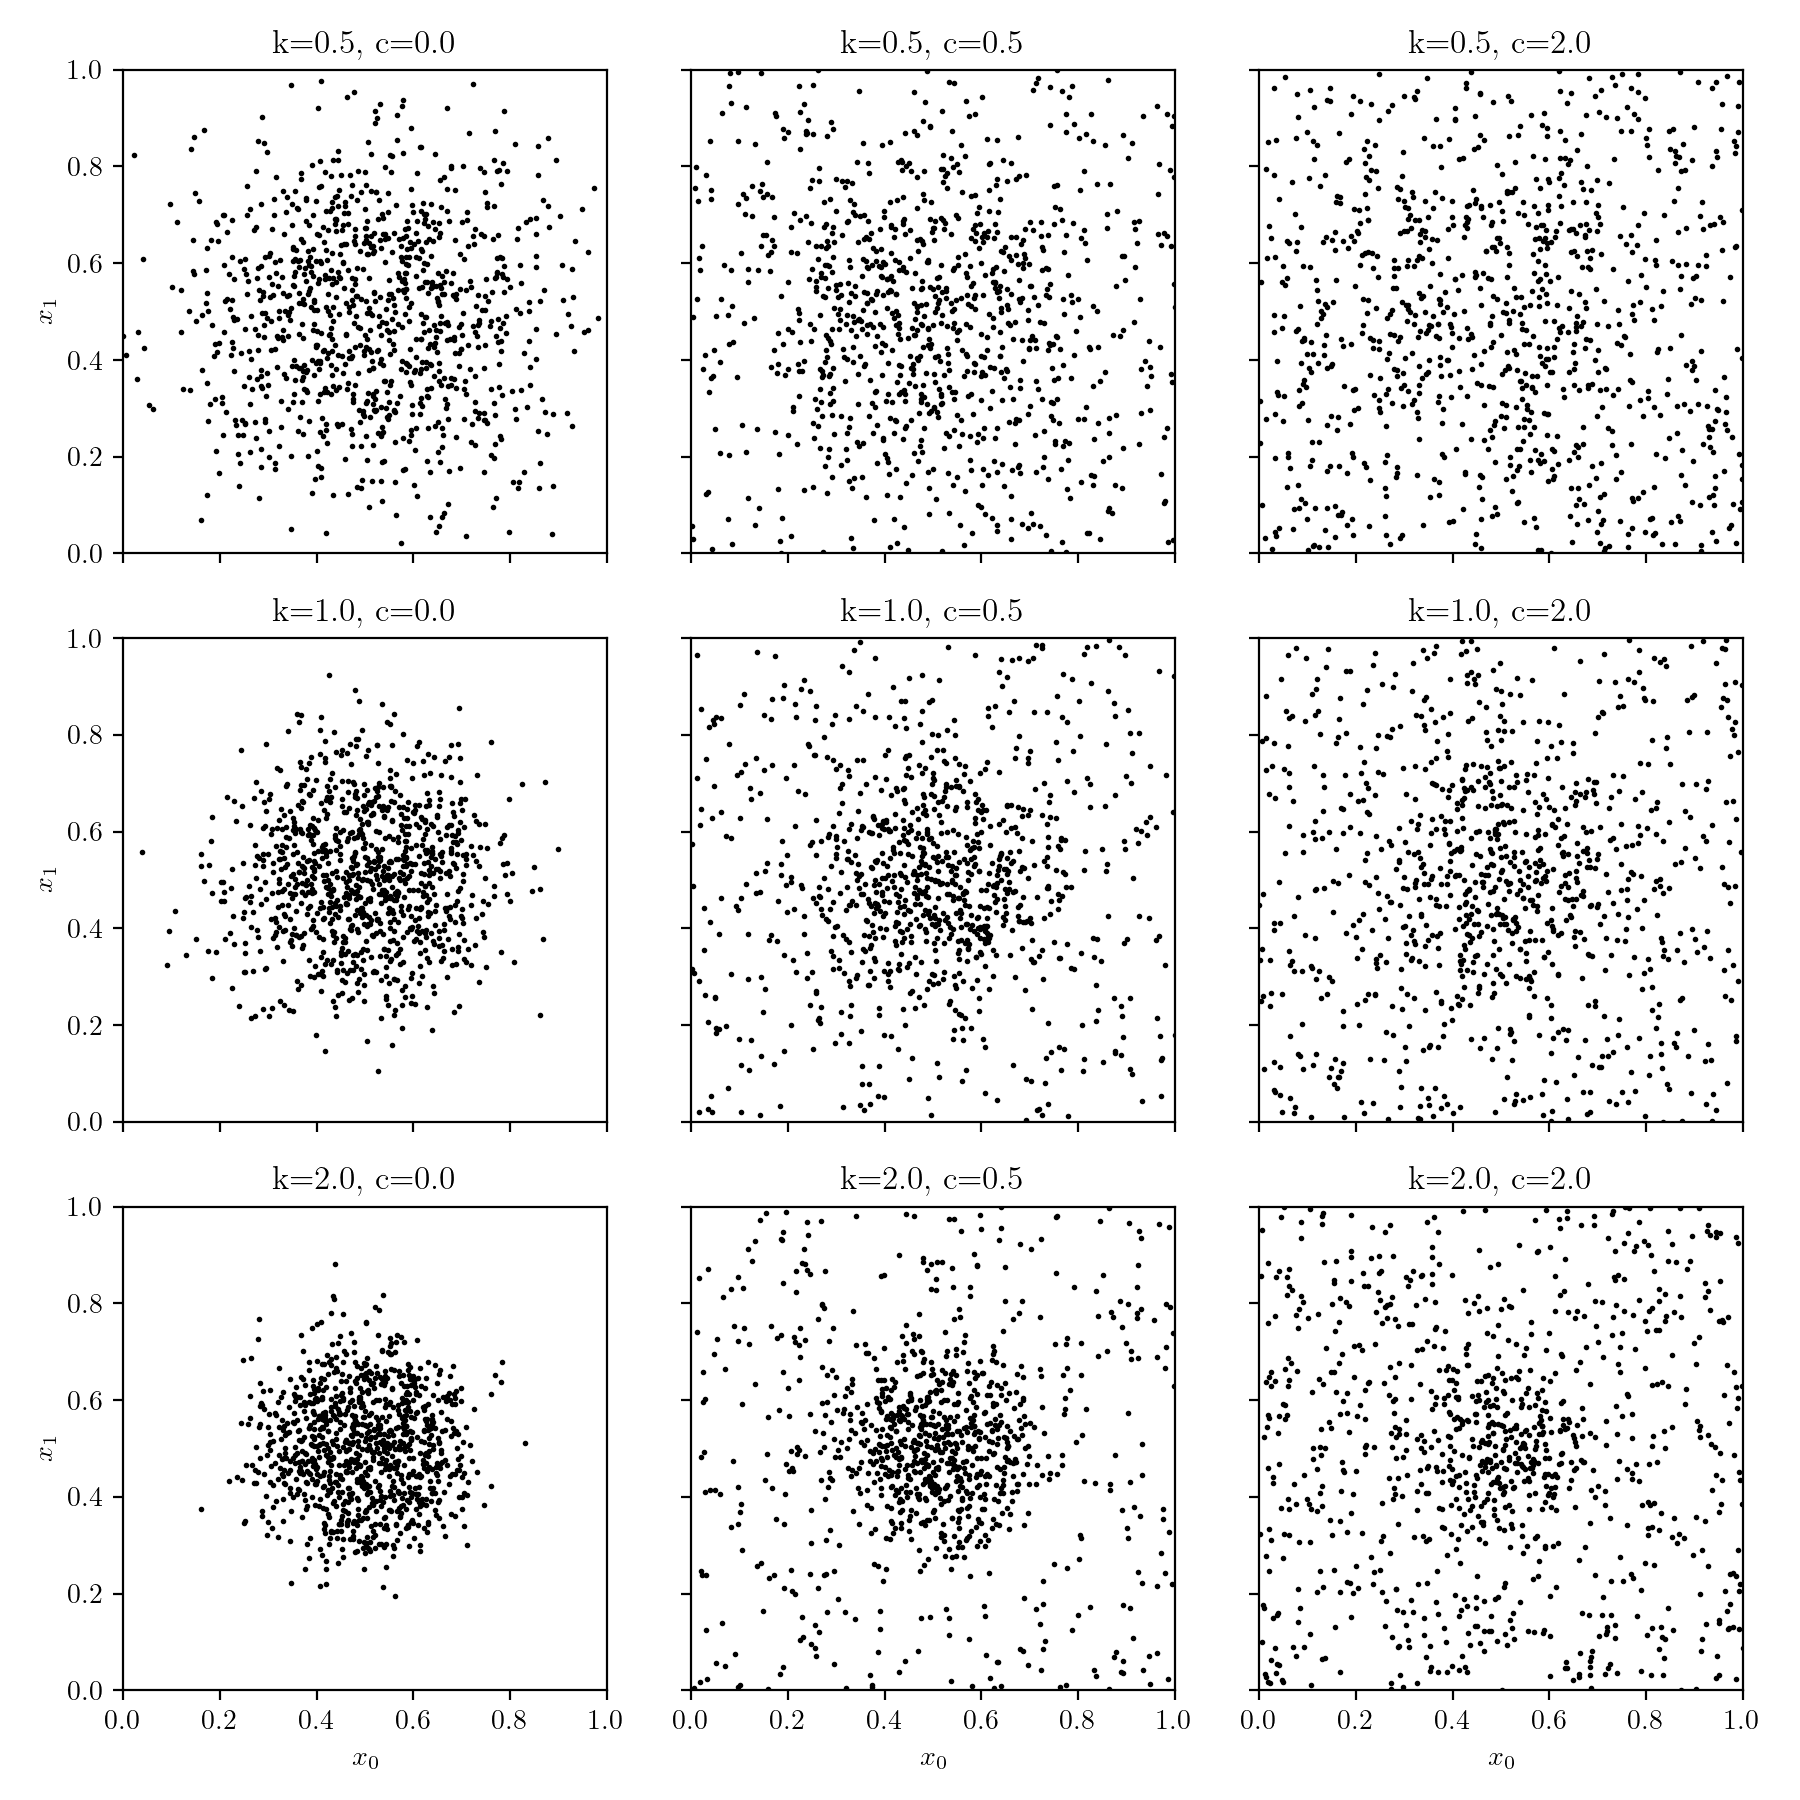
\includegraphics[width=150mm]{figures/sampling_kc.png}
    \caption{RAR-D}
    \label{fig:rar-d}
\end{figure}


%\subsubsection{Langevin dynamics - TD}
%(NeurIPS 2025)
%sample the domain
%treat point movements as langevin dynamics 
%- add noise
%- movements based on residual forces
%
%\subsubsection{TD}
%sample using LHC up front - 10,000 - 100,000, bc and ic = pde / 10
%n epochs = 10,000 - 20,000
%new sample every 500 epochs
%    - entire new LHC sample, or
%    - entire new LHC sample based on residuum (RAR / RAD-distribution)
%also can try: RAR-D (RAR + Distribution):
%    - keep top 30percent of highest-residual points, resample the rest with RAD weights.
%

\subsubsection{SDE sampling}
Euler Maruyama



\subsection{Appoximating the spatial derivatives}

\subsubsection{Stochastic Dimension Gradient Descent (SDGD)}
% https://arxiv.org/html/2307.12306v5#S3

SDGD approximates the loss by decomposing the PDE operator into dimension-wise terms, sampling subsets during training.
This dramatically decreases the memory requirements of AD and theoretically unlocks it to very high dimensions ($\sim 100$).

Consider a linear PDE of the form:
$$
\mathcal{L}u(x) = f(x)
$$
where, $\mathcal{L}$ is a differential operator, for example,

$$
\mathcal{L} = \sum_{i=1}^d\frac{\partial^2}{\partial x_i^2}\;,\quad\text{or}
$$
$$
\mathcal{L} = \sum_{i,j=1}^d\frac{\partial^2}{\partial x_i \partial x_j} + \sum_{i=1}^d a_i\frac{\partial}{\partial x_i}
$$

In general, we can split the operator into $n$ independent parts $\mathcal{L} = \sum_{i=1}^n\mathcal{L}_i$.
For the two examples given above, this could be
$$
\mathcal{L} = \sum_{i=1}^d \mathcal{L}_i
\quad \text{where}\quad
\mathcal{L}_i = \frac{\partial^2}{\partial x_i^2}
\quad \text{and} \quad n=d
$$
$$
\mathcal{L} = \sum_{i,j=1}^d \mathcal{L}_{ij}
\quad \text{where}\quad
\mathcal{L}_{ij} = \frac{\partial^2}{\partial x_i\partial x_j} + \frac{a_i}{d} \frac{\partial}{\partial x_i}
\quad \text{and} \quad n=d^2
$$

We can therefore write
$$
\sum_{i=1}^n\mathcal{L}_i u(x) = f(x)
$$

Now consider a PINN approximation $u_\theta \approx u$. 
The pde loss at a point $x\in\mathbb{R}^d$ can then be written in the form

$$
\ell_{pde}(\theta;x)
= \big( \mathcal{L} u_\theta(x) - f(x) \big)^2
= \left( \sum_{i=1}^n \mathcal{L}_i u_\theta(x) - f(x) \right)^2
$$

And the corresponding gradient w.r.t. the model weights is then

$$
\nabla_\theta \ell_{pde}(\theta;x) = \nabla_\theta \left( \sum_{i=1}^n \mathcal{L}_i u_\theta(x) - f(x) \right)^2
= 2 \left( \sum_{i=1}^n \mathcal{L}_i u_\theta(x) - f(x) \right) \left( \sum_{i=1}^n \nabla_\theta \mathcal{L}_i u_\theta(x) \right)
$$

Finally, we consider a subset $I \subset \{1, \dots, n\}$ with $|I| \ll n$, and approximate the last term from the equation above,
$$
\left( \sum_{i=1}^n \nabla_\theta \mathcal{L}_i u_\theta(x) \right)
$$
as
$$
\frac{n}{|I|} \left( \sum_{i \in I} \nabla_\theta \mathcal{L}_i u_\theta(x) \right)
$$


In the context of the training loop, SDGD is implemented as follows:

\begin{enumerate}
%\item consider some point $x\in\mathbb{R}^{d}$
\item consider some batch of points $X\in\mathbb{R}^{bs\times d}$
\item sample index set $I \subset \{1, \dots, n\}$ with $|I| \ll n$
\item compute $\mathcal{L}_i u_\theta(X)$ for all $i=1,\dots,n$ and detach the computational graph behind the terms $i\notin I$ from memory
\item backpropagate only through terms $i \in I$ as so:
$$
\nabla_\theta \ell_{pde}^I(\theta;X) = 2\,\frac{n}{|I|} \left( \sum_{i=1}^n \mathcal{L}_i u_\theta(X) - R \right) \nabla_\theta \left( \sum_{i \in I} \mathcal{L}_i u_\theta(X) \right)
$$
\end{enumerate}

the other $i\notin I$ are treated as scalars

%$$
%\mathbb{E}_I [\nabla_\theta \ell_{pde}^I] = \nabla_\theta \ell_{pde}
%$$
%(memory $O(|I|)$ vs. $O(n)$) 



%For multiple points $\{\mathbf{x}_n\}_{n=1}^{N_r}$, normalize $\frac{1}{N_r N_L^2} \sum_n (\cdot)^2$;
%joint batches B over points,
%I over terms yield $g_{B,I}(\theta) = \frac{1}{|B| |I| N_L} \sum_{n \in B} (\sum_i \mathcal{L}_i u_\theta(\mathbf{x}_n) - R) \sum_{i \in I} \partial_\theta \mathcal{L}_i u_\theta(\mathbf{x}_n)$
%
%Unbiasedness: Proven via linearity of expectation.
%
%Variance: $V_{B,I}[g_{B,I}] = \frac{C_1}{|B|} + \frac{C_2}{|I|} + \frac{C_3}{|B| |I|}$, minimized under fixed memory $|B| \times |I|$ by balancing point/term variance (e.g., equal for comparable $C_1, C_2$).
%
%Bounded variance/convergence: Under smooth activations ($|\sigma^{(k)}| \leq 1$, Lipschitz), variance $O(h^{2n} N_L R^2 / |B| |I|)$ (h: width, n: order); SGD converges as $\mathcal{O}(1/\sqrt{T})$ with stepsize decay
%
%1. Sample I, compute/detach all $\mathcal{L}_i u_\theta$.
%
%2. Backprop $i \in I$, form $\nabla_\theta \ell_I$.
%
%3. Update $\theta \leftarrow \theta - \eta \nabla_\theta \ell_I$


\subsubsection{Hutchinson trace estimation (HTE)}
% https://arxiv.org/html/2312.14499v2#S3
Consider a symetric positive semidefinite matrix $A\in\mathbb{R}^{n\times n}$.
The trace of $A$ can be approximated as an expectation
$$
tr(A) = \mathbb{E}_{v\sim\rho}[v^T A v]
$$
where $v$ is a random vector satisfying $\mathbb{E}_{v\sim\rho}[vv^T] = I$.
The distribution $\rho$ can be chosen as normal.
However, Hutchinson's original paper, and now the standard choice, is a Rademacher distribution, where the entries of a vector $v$ are chosen as $\pm 1$ with probability $\frac{1}{2}$.

The Rademacher distribution is the prefered choice as it gives an optimal variance of this estimator.
It also requires a relatively few samples, on the order of 10s, 100s, to converge to within a relative error of 0.1, 0.01 respectively.

In the context of PINNs, we can take $A = \text{Hess}(u) := \frac{\partial^2 u}{\partial x_i \partial x_j}$,
and by approximating $tr(A)$, we get an approximation for $\Delta u$.


% variance
% 1 https://claude.ai/share/4af41507-635c-43b2-8a24-df228ff808fb
% variance odvozeni:
% 2 https://www.ethanepperly.com/index.php/2023/01/26/stochastic-trace-estimation/#real-gaussians
% rigorous error estimates:
% 3 https://dl.acm.org/doi/epdf/10.1145/1944345.1944349
% Variance for a single $v\sim\mathcal{N}(0,1)$:
% $$
% Var(v^T A\,v) = 2||A||_F^2
% $$
% Variance for a single $v\sim\rho_{Rademacher}$:
% $$
% Var(v^T A\,v) = 2||A||_F^2 - 2\sum_i A_{ii}^2
% $$

\subsection{Loss weighting}

Grad Norm
- compute grad of norms of loss
%https://pmc.ncbi.nlm.nih.gov/articles/PMC12858974/#:~:text=The%20loss%20function%20in%20PINNs,adaptive%20loss

SoftAdapt
% https://arxiv.org/pdf/2009.04544v5
% https://github.com/levimcclenny/SA-PINNs
- learnable attention params

\section{Causal training}

In the original PINN architecture, time is handled just as another input dimension without any special treatment.
But since its incepetions it became apparant that this threatement is not adequete in some cases
When training PINNs on time-dependent PDEs, the optimizer minimizes the residual over all time steps simultaneously.
This can lead to causality violation: the network attempts to fit later-time dynamics before earlier-time states are correctly learned, producing globally low residual but physically meaningless solutions.
%\cite{causal_pinns}

Thus a few competing strategies have emerged as a viable alternatives to the original formulation.

\subsection{Time marching}
One simple approach is to divide the interval into multiple segments and train a PINN for each one.
%\cite{time_adaptive_pinns}
The networks have to be trained in series, as the intial considiton for the $k$-th network is taken as the terminal state of the $k-1$-th network.

\subsection{Time-adaptive sampling}
Here, we train the neural network on a ever increasing temporal domain.
sample in interval $[0,\tau t], \tau\sim \frac{step}{n_steps}T$

%\cite{time_adaptive_pinns}


\subsection{Causal weighting}
% Wang et al., "Respecting Causality is All You Need" / experts guide
% also note that large batches are good for hard problems - enhanced convergence and accuracy
% - but gpus not enough memory
% - split large batch into smaller subbatches, parallelize loss compute across gpus
% - compute grad desc. on all
% - average model param update

Causal weighting addresses this by partitioning the time domain $[0,T]$ into $M$ ordered segments
$[t_{m-1}, t_m),\:m=1,\dots,M\,,\:
0 = t_0 < t_1 < \cdots < t_M = T,
$ and computig the pde loss as

$$
\ell_{pde} = \frac{1}{M}\sum_{m=1}^{M} w_m\, \ell_{pde}^{(m)}
$$

where
$\ell_{pde}^{(m)}$
is the loss computed from the points falling in the $m$-th time segment $[t_{m-1}, t_m)$, 
and the causal weight $w_m$ for segment $m$ is an exponential weight that depends on the cumulative residual of all preceding segments:
$$
w_m = \exp\!\Biggl(-\varepsilon \sum_{k=1}^{m-1} \ell_{pde}^{(k)}\Biggr)
\,,\quad m=2,\dots,M
$$
$$
w_m = 1
\,,\quad m=1
$$
Here, $\varepsilon > 0$ is a causality parameter controlling the strictness of the temporal ordering.
When $\varepsilon = 0$, all segments are weighted equally (standard training).
As $\varepsilon \to \infty$, the training concentrates entirely on the earliest segment whose residual has not yet converged.


All $w_m$ intiialize by 1

Note that the weights $w_m$ are detached from the computational graph, that is, the backward pass sees them only as scalars with no computation graph behind them.



\subsection{Problem specific technique - Capturing physics}
add additional residuals capturing the physics
- symmetries, energy conserv, ...

use problem symmetries
- separability
- prob? do in log space
- en conservation?

transfer learning - traing on easier problem, then more to the harder one

researchers (Liu and Gerstoft, 2023) have ensured that the model strictly
adheres to specific physical laws by introducing additional physical
constraints, such as conservation laws, temporal invariance, and spatial
smoothing into the loss function. This approach significantly enhances
the accuracy and stability of the model. For instance, Zhang (Zhang
et al., 2023a) incorporated invariance conditions derived from Lie
symmetry into the loss function, improving t

exp(NN) -> u > 0 (prob)




\subsection{Other}

\subsubsection{Hard constrains}
architectuary enforce IC and BC - nn then need to learn only the pde
% https://arxiv.org/html/2404.16189v3#:~:text=as%20the%20IC%20data%20is,We%20consider%20the%20following%20transformation

weight intialization (Glorot)

normalize input: [-1,1] or [0,1]


activations - tanh / silu (smooth)
$$
silu(x) = x \cdot \sigma(x)
$$

NNs learn low freq sol first


\subsubsection{Random Fourier features}

As reported by , neural networks are biased for learning low frequency signals first
before proceeding to learn high freq ones.
\cite{experts_guide}

In 2019, Rahaman et al.
consider uniform distributio of training data
learn low freq smooth patterns before high freq ones
learn low freq first even when high freq have large amplitudes
low freq stable when perturbing netwrork params
consider nns with relu activations trained via gradient descent
use fourier analysis
call this phenomena spectral bias
\cite{spectral_bias_relu}

More interesting for our case:
extends to non-uniform data - in the context of pinns - one region sampled more than other
use NTK (Neural Tanget Kernel) theory
- looks at $K(x_i,x_j)=
<\frac{\partial NN_\theta(x_i)}{\partial \theta},
<\frac{\partial NN_\theta(x_j)}{\partial \theta}>$
consider training for harmonic target function with freq $\kappa$
speed of training convergence at a points $x$ is proportial to
$O(\frac{\kappa^d}{p(x)})$ where $p(x)$ is a local data density
$d$ - input dimension of the NN
\cite{freq_bias_NTK}

solution coming from computer vision
$$
\gamma(x) =
\begin{pmatrix}
    \cos(2\pi B x)\\
    \sin(2\pi B x)
\end{pmatrix}
$$
$B\in\mathbb R^{m\times d}$ sampled from Gaussian distribution $\mathcal N(0,\sigma^2)$
spatial / tempotal
\cite{fourfeat}


%\subsubsection{Random Weight Factorization}
%% arXiv:2308.08468, Sec 4.3
%
%Standard PINN training often suffers from slow convergence due to the loss landscape geometry.
%Random Weight Factorization (RWF) \cite{rwf_modified_mlp} reparametrizes each weight matrix by factoring it into a diagonal scale matrix and a weight factor:
%$$
%W^{(l)} = \operatorname{diag}\!\bigl(\exp(s^{(l)})\bigr)\, V^{(l)}, \qquad l = 1,\dots,L{+}1,
%$$
%where $s^{(l)} \in \mathbb{R}^{d_l}$ is a trainable scale vector and $V^{(l)} \in \mathbb{R}^{d_l \times d_{l-1}}$ is the corresponding weight factor.
%The exponential parametrization ensures that the per-neuron scales remain strictly positive and can span a wide range of magnitudes.
%
%The initialization proceeds as follows:
%\begin{enumerate}
%    \item Initialize a weight matrix $W^{(l)}$ via Glorot (Xavier) initialization.
%    \item Sample the scale vector $s^{(l)} \sim \mathcal{N}(\mu,\, \sigma^2 I)$, with recommended defaults $\mu = 1.0$, $\sigma = 0.1$.
%    \item Set $V^{(l)} = \operatorname{diag}\!\bigl(\exp(-s^{(l)})\bigr)\, W^{(l)}$, so that the effective weight $\operatorname{diag}(\exp(s^{(l)}))\, V^{(l)} = W^{(l)}$ matches the original Glorot initialization.
%\end{enumerate}
%The trainable parameters per layer are $\{s^{(l)},\, V^{(l)},\, b^{(l)}\}$.
%During the forward pass, the output of each layer is computed efficiently as
%$$
%y = \bigl(x\, {V^{(l)}}^\top\bigr) \odot \exp(s^{(l)}) + b^{(l)},
%$$
%without materializing the full weight matrix $W^{(l)}$.
%The factorization introduces additional degrees of freedom in the loss landscape, which helps the optimizer escape saddle points and accelerates convergence, particularly for multi-scale PDE solutions.
%
%
%\subsubsection{Modified MLP}
%% arXiv:2308.08468, Sec 6.4 (Wang et al.)
%
%A known limitation of standard MLPs in the PINN setting is that input information is progressively diluted through successive layers, making it difficult for deeper layers to retain sensitivity to the original coordinates.
%The Modified MLP \cite{rwf_modified_mlp} addresses this by introducing two encoder sub-networks whose outputs are injected into every hidden layer via element-wise gating.
%
%Given input $x \in \mathbb{R}^{d_{\mathrm{in}}}$, two encodings are computed:
%$$
%U = \sigma(W_1\, x + b_1), \qquad V = \sigma(W_2\, x + b_2),
%$$
%where $W_1, W_2 \in \mathbb{R}^{h \times d_{\mathrm{in}}}$, $b_1, b_2 \in \mathbb{R}^h$, and $\sigma$ is the activation function (e.g.\ $\tanh$).
%
%The hidden layers are then defined recursively. Starting from $g^{(0)} = x$, for $l = 1, \dots, L$:
%\begin{align}
%    f^{(l)} &= W^{(l)}\, g^{(l-1)} + b^{(l)}, \\
%    g^{(l)} &= \sigma\!\bigl(f^{(l)}\bigr) \odot U \;+\; \bigl(1 - \sigma\!\bigl(f^{(l)}\bigr)\bigr) \odot V,
%\end{align}
%where $\odot$ denotes element-wise multiplication.
%The final output is a standard linear projection:
%$$
%u_\theta(x) = W^{(L+1)}\, g^{(L)} + b^{(L+1)}.
%$$
%
%The gating mechanism $\sigma(f^{(l)}) \odot U + (1 - \sigma(f^{(l)})) \odot V$ acts as a learned interpolation between the two input encodings at each layer, ensuring that the network retains direct access to input-derived features at every depth.
%Both techniques can be combined: RWF can be applied to all weight matrices in the Modified MLP, including the encoder matrices $W_1$ and $W_2$.
%
%
%XPINN - mulitple pinns - overlapping domains
%
%PDE separable? -> sum of product of 1d networks

\subsection{L-BFGS}
limited memory
quasi newton

\subsection{my genious ideas TD}
- have 3 networks - each focused on different frequency signals

- extreme machine learning
(periodically give a LLM during the training a snapshot of the loss, the l2, l1 errs and give it some params to tweak)



\section{Optimization}


\subsection{GPU-CPU orchestration / term-by-term}
- torch.profiler and chrome

\subsection{GPU memory requirements of the loss computation}
- benchmarks:
    - normal
    - HTE
    - sdgd
- observe:
    - peak memory
    - timeseries memory
    - time

sample X

pde terms computation
- forward: u(X)
- grad of u
- other terms
- summ together

loss = sum batch vals together and l2

backpropagate?


- float32 / float64

\subsection{hardware}
- n of gpus
- vRAM

\subsection{software}
- jax prob better
- torch for arch
- AD - jacrev,... - jax like



\section{Experiments}

- memory footprint of AD
    - grad u
    - laplace u
    - div(A grad u)
    - hessian u


\section{grid search exploration}
importance of weights of losses
    - hard constrains
    - fixed losses
    - adaptive loss weighting via GradNorm





\chapter{Conclusion}

speed and precision still on the side of sparse grids?

established convergence theory

pinns - hyperparameter tuning





\section{Math recap}

Positive semidefinite matrix $A\in\mathbb{R}^{n \times n}$ is a symmetric matrix, that satisfies:
$$ x^T A\,x \ge 0, \quad \forall x\in\mathbb{R}^n, \: x\neq 0 $$



\cite{experts_guide}
\cite{systematic_review}




